
\subsubsection*{Kali Linux}
Kali Linux es una distribución de Linux (basada en Debian) centrada en la seguridad. 
Es una versión renombrada de la famosa distribución de Linux conocida como Backtrack, 
que venía con un enorme repositorio de herramientas de piratería de código abierto, 
para pruebas de penetración de aplicaciones web, inalámbricas y de red. Aunque Kali 
Linux contiene la mayoría de las herramientas de Backtrack, el objetivo principal 
de Kali Linux es hacerlo portátil para que pueda instalarse en dispositivos basados 
en arquitecturas ARM como tabletas y Chromebooks.

\begin{center}
    \begin{figure}   
       \begin{center}
          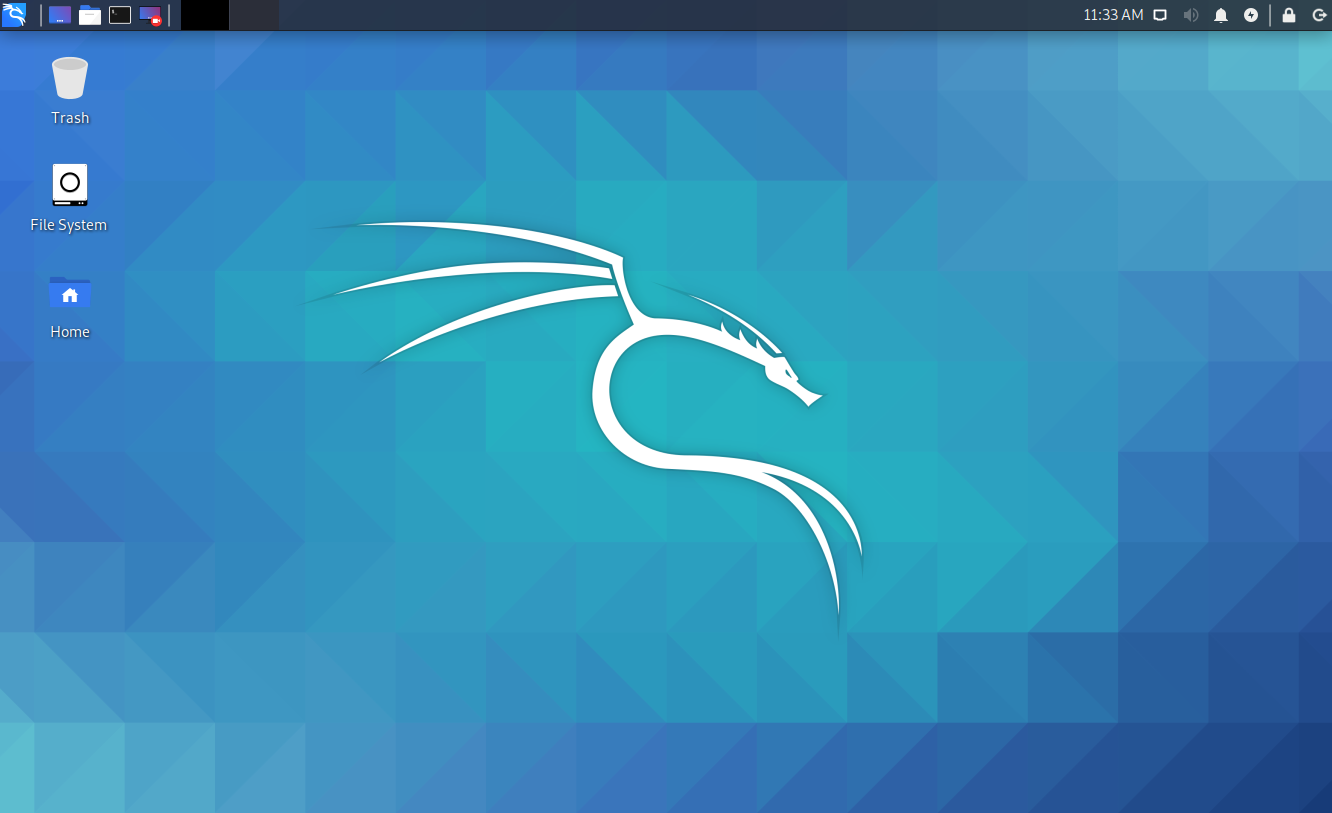
\includegraphics[width=11cm,height=7cm]{ataque-1.png}
       \end{center}
       \caption{Escritorio de Kali Linux}
    \end{figure}
 \end{center}
 

El uso de herramientas de piratería de código abierto tiene un gran inconveniente: 
contienen una gran cantidad de dependencias cuando se instalan en Linux y deben 
instalarse en una secuencia predefinida. Además, los autores de algunas herramientas 
no han publicado documentación precisa, lo que aumenta la dificultad.

Kali Linux simplifica este proceso; contiene muchas herramientas preinstaladas con 
todas las dependencias y ya está lista para usar. Esto nos permite tener que prestar 
más atención al ataque real y no a la instalación de la herramienta. Las actualizaciones 
para las herramientas instaladas en Kali Linux se publican con mayor frecuencia, 
lo que le ayuda a mantener las a las mismas actualizadas.

Este sistema operativo contiene las herramientas necesarias para realizar nuestro
pequeño ataque, las mismas serán nombradas a continuación.

\subsubsection*{Wireshark}
Wireshark es uno de los analizadores de protocolos de red más populares, es de 
código abierto y gratuito. Wireshark está preinstalado en Kali y es ideal para la 
resolución de problemas de red, análisis y, para este caso de estudio, una herramienta 
perfecta para monitorear el tráfico de posibles objetivos. Wireshark usa un kit de 
herramientas para implementar su interfaz de usuario y para capturar paquetes. 
Funciona de manera muy similar a un comando \emph{tcpdump}; sin embargo, actúa al contener 
una interfaz gráfica, tiene opciones integradas de clasificación y filtrado.

\begin{center}
    \begin{figure}   
       \begin{center}
          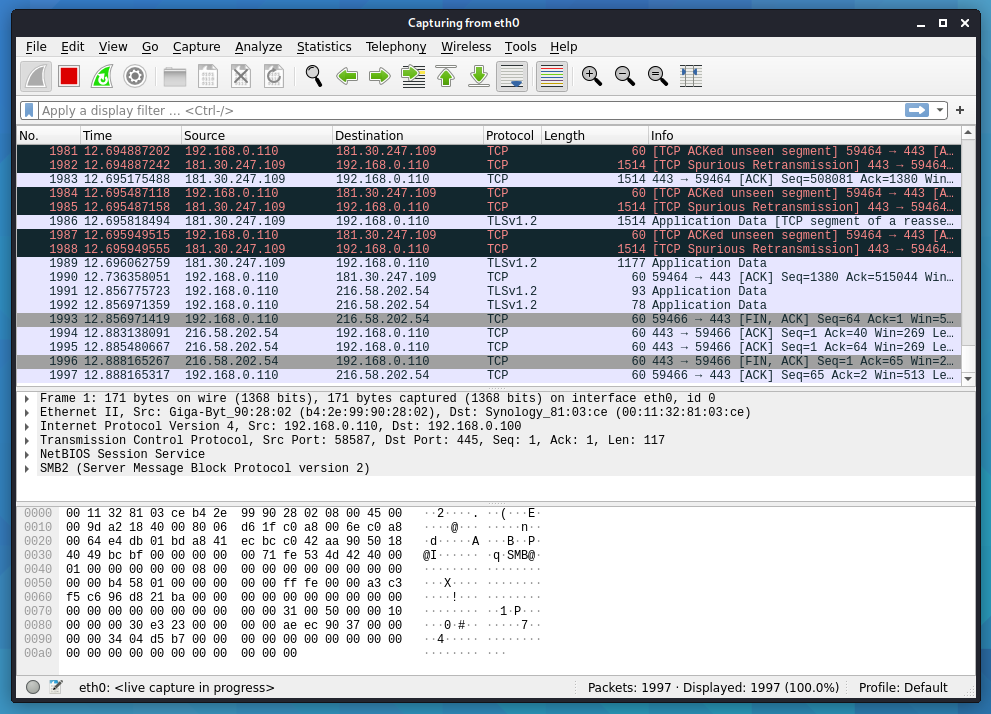
\includegraphics[width=10cm,height=7cm]{wireshark.png}
       \end{center}
       \caption{Interface del Wireshark}
    \end{figure}
 \end{center}
 
\subsubsection*{Ettercap}

Ettercap es un paquete completo gratuito y de código abierto para ataques basados 
en intermediarios. Ettercap se puede utilizar para análisis de protocolos de redes 
informáticas y auditorías de seguridad, con funciones de rastreo de conexiones en 
tiempo real y filtrado de contenido. Ettercap funciona poniendo la interfaz de red 
del atacante en modo promiscuo y ARP para envenenar las máquinas víctimas.

